\documentclass[11pt,aspectratio=43,usenames,dvipsnames]{beamer}
\usepackage[utf8]{inputenc}
\usepackage{amsmath, amsfonts, amssymb, amsthm}
\usepackage[T1]{fontenc}
% mint: code chuck and syntax highlighting
%% outputdir should change according to pdf build directory
\usepackage[outputdir=build,cache=false]{minted}
\usepackage{lmodern}
\usepackage{xcolor}
\usepackage{setspace}
\usepackage{booktabs}
\usepackage{multirow}
\usepackage{graphicx}
\usepackage{fontawesome}

\usepackage[mode=tex]{standalone}

\usepackage{tikz}
\usetikzlibrary{decorations}
\usetikzlibrary{decorations.pathreplacing, intersections}
\usepackage{pgfplots}
\usetikzlibrary{calc,positioning}
\usepgfplotslibrary{fillbetween}
\pgfplotsset{compat=newest, scale only axis, width = 10cm}

\newcommand{\kora}{%
(\raisebox{0.5em}{\rotatebox{-45}{)}}$^{\circ}{\scriptscriptstyle\Box}^{\circ}$)\raisebox{0.5em}{\rotatebox{-45}{)}}\rotatebox{90}{)}\raisebox{0.2em}{\LARGE \_\hskip-.1em\textvisiblespace\hskip-.1em\_}
}

% ---------------------------------------------------------------------
% Coordinate extraction
% #1: node name
% #2: output macro name: x coordinate
% #3: output macro name: y coordinate
\newcommand{\Getxycoords}[3]{%
    \pgfplotsextra{%
        % using `\pgfplotspointgetcoordinates' stores the (axis)
        % coordinates in `data point' which then can be called by
        % `\pgfkeysvalueof' or `\pgfkeysgetvalue'
        \pgfplotspointgetcoordinates{(#1)}%
        % `\global' (a TeX macro and not a TikZ/PGFPlots one) allows to
        % store the values globally
         \global\pgfkeysgetvalue{/data point/x}{#2}%
         \global\pgfkeysgetvalue{/data point/y}{#3}%
     }%
}
% ---------------------------------------------------------------------

\usepackage{ulem}
\usepackage{hyperref}
\usepackage{booktabs}
\usepackage{babel}
\usepackage{makecell}
\usepackage[para,online,flushleft]{threeparttable}
\usepackage{pdfpages}
\usepackage{tcolorbox}
\usepackage{bm}
\usepackage{appendixnumberbeamer}
\usepackage{natbib}
\usepackage{caption}
\captionsetup[figure]{labelformat=empty}% redefines the caption setup of the figures environment in the beamer class.
\usetheme[compress]{Boadilla}
\usecolortheme{default}
\useoutertheme{miniframes}
\usefonttheme[onlymath]{serif}

\newcommand{\jump}[2]{\hyperlink{#1}{\beamerbutton{#2}}}
\newcommand{\orange}[1]{\textcolor{orange}{#1}}
\newcommand{\red}[1]{\textcolor{red}{#1}}
\newcommand{\blue}[1]{\textcolor{blue}{#1}}
\newcommand{\green}[1]{\textcolor{OliveGreen}{#1}}

\renewcommand{\square}{\scalebox{0.7}{$\blacksquare$ \hspace{0.5em}}}
\setbeamertemplate{itemize item}{\raisebox{0.1em}{\scalebox{0.7}{$\blacksquare$}}}
\setbeamertemplate{itemize subitem}[circle]
\setbeamertemplate{itemize subsubitem}{--}
\setbeamercolor{itemize item}{fg=black}
\setbeamercolor{itemize subitem}{fg=black}
\setbeamercolor{itemize subsubitem}{fg=black}
\setbeamercolor{item projected}{bg=darkgray,fg=white}
\definecolor{blue}{rgb}{0.2, 0.2, 0.7}
\setbeamercolor{alerted text}{fg=blue}
\setbeamertemplate{enumerate items}[circle]


\setbeamertemplate{headline}{}

%==========================================
\let\olditemize=\itemize
\let\endolditemize=\enditemize
\renewenvironment{itemize}{\olditemize \itemsep1em}{\endolditemize}
\let\oldenumerate=\enumerate
\let\endoldenumerate=\endenumerate
\renewenvironment{enumerate}{\oldenumerate \itemsep1em}{ \endoldenumerate}

\DeclareMathOperator*{\argmax}{\arg\!\max}
\DeclareMathOperator*{\E}{\mathbb{E}}
\DeclareMathOperator*{\var}{\rm Var}
\DeclareMathOperator*{\cov}{\rm Cov}

\theoremstyle{definition}
\newtheorem{assume}{Assumption}
\newtheorem{lem}{Lemma}
\newtheorem{proposition}{Proposition}
\newtheorem{thm}{Theorem}
\newtheorem{corol}{Corollary}

\AtBeginSection[]{
  \begin{frame}[noframenumbering]
  \vfill
  \centering
  \begin{beamercolorbox}[sep=8pt,center,shadow=true,rounded=true]{title}
    \usebeamerfont{title}\insertsection\par%
  \end{beamercolorbox}
  \vfill
  \end{frame}
}

\begin{document}
    \title[Unit 9]{Unit 9: \\ The Labor Market, \\ Wages, Profits, and Unemployment}
    \author[Hui-Jun Chen]{Hui-Jun Chen}
    \institute[OSU]{The Ohio State University}
    % \date{\today}
    \date{\today}
    \setbeamertemplate{navigation symbols}{}
    \setstretch{1.2}

%-------------------------------------------------------
{
%	\usebackgroundtemplate{\includegraphics[width=1\paperwidth]{../EveningSky_cropped_edit43_bright.jpg}}
    \begin{frame}
% \vspace{3em}
        \centering
%		{\footnotesize 	ECON 4002 Intermediate Macroeconomic Theory}
        \maketitle
% \vspace{-1.5em}
% \centering
% \includegraphics[width=0.55\linewidth]{Pictures/houses.jpeg}


    \end{frame}
}

% -------------------------------------------
\setbeamertemplate{headline}
{
\setbeamercolor{section in head/foot}{fg=black, bg=white}
\vskip1em \tiny \insertsectionnavigationhorizontal{1\paperwidth}{\hspace{0.50\paperwidth}}{}
}
%------------------------------------------

\section[Intro]{Introduction}
\label{sec:Introduction}

\begin{frame}{Introduction}
\label{slide:Introduction}

\begin{center}
    \textit{How is economy-wide wage and unemployment determined?}
\end{center}

\begin{itemize}
    \item Until now we are analyzing equilibrium in \alert{goods market}.
    \item \alert{Labor market} connectes with firms' performance in goods market:
    \begin{itemize}
        \item Goods market price high $ \Rightarrow  $ firm earns profit $ \Rightarrow  $ wage increases $ \Rightarrow  $ more hiring $ \Rightarrow  $ unemployment $ \downarrow  $ $ \Rightarrow  $ demand for good is higher, market price higher
    \end{itemize}
    \item Since we have solved the goods market, we are going to use goods market result to solve the relationship between \alert{wage} and \alert{unemployment rate}:
    \begin{itemize}
        \item wage-setting curve: relationship between firm and \alert{employees}
        \item price-setting curve: relationship between firm and \alert{consumers}
    \end{itemize}
\end{itemize}

\end{frame}

\section[Unemployment]{Measuring Unemployment}
\label{sec:Measuring_Unemployment}

\begin{frame}{Unemployment Definition}
\label{slide:Unemployment_Definition}
    The unemployed are the people who are not in \alert{paid employment or self-employment}, \alert{available} for work, and \alert{actively seeking} work.
    \begin{itemize}
        \item not available for work: students, institutionalized, retired, children
        \item not actively seeking: not seeking for the 4 weeks (BLS)
        \item might subject to definition by researchers
    \end{itemize}
\end{frame}

\begin{frame}{Population Sections and Rate definition}
\label{slide:Population_Sections}
    \begin{figure}
        \centering
        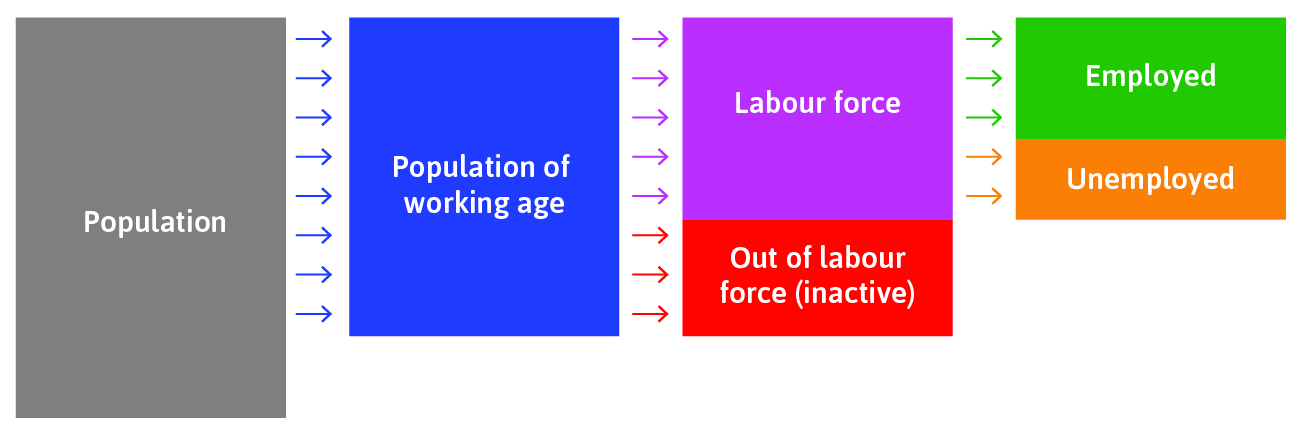
\includegraphics[width=\textwidth]{./figures/employmentPop.jpg}
    \end{figure}

    \begin{itemize}
        \item participation rate $ =  \frac{\text{labor force}}{\text{population of working age}}$
        \item unemployment rate $ = \frac{\text{unemployed}}{\alert{\text{labor force}}} $
        \item employment rate $ = \frac{\text{employed}}{\alert{\text{population of working age}}} $
        \item Why?! \faFrownO
    \end{itemize}

\end{frame}

\section[P\&W]{Price-Setting and Wage-Setting}
\label{sec:Price_Setting_and_Wage_Setting}

\begin{frame}{Real Wage / Relative Price}
\label{slide:Real_Wage___Relative_Price}
    The real wage is the nominal wage divided by the price level of the bundle of consumer goods purchased.

    %
    \begin{equation*}
        w = \frac{W}{P}
    .\end{equation*}
    %
    \begin{enumerate}
        \item each firm decides on its: price, wage, how many people to hire
        \item adding up all of these across all firms gives the total employment in the economy and the real wage
    \end{enumerate}

\end{frame}

\begin{frame}{Firm's Decision}
\label{slide:Firm_s_Decision}

\begin{itemize}
    \item Unemployment rate is the aggregated outcome of individual firms/workers' decisions.
    \item With labor discipline model, how does the reservation wage change with unemployment rate?
    \item \alert{unemployment rate $ \uparrow  $} $ \Rightarrow  $ gov's unemployment benefit per person $ \downarrow  $, given fixed budget $ \Rightarrow  $ \alert{worker's reservation wage $ \downarrow  $}
    \item $ \Rightarrow  $ shift worker's best response curve to the \alert{left}
\end{itemize}
\end{frame}

\begin{frame}{Shift in wage-setting curve}
\label{slide:Shift_in_wage_setting_curve}
    \begin{figure}
        \centering
        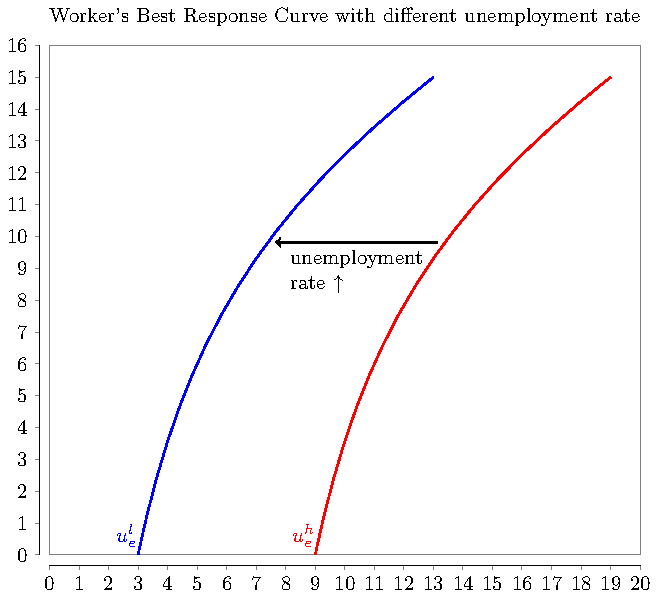
\includegraphics[width=0.7\textwidth]{../Unit6FirmLaborMarket/figures/BestResponse}
    \end{figure}

\end{frame}


\begin{frame}{Aggregation for Wage-setting curve}
\label{slide:Aggregation_for_Wage_setting_curve}
    \begin{center}
    \begin{tikzpicture}[scale = 0.9]
        \pgfmathsetmacro{\x}{10}
        \pgfmathsetmacro{\y}{7}
        % \draw[very thin,color=gray] (0,0) grid (\x, \y); % gray grid
        \draw[->] (0, 5) node[below]{ $ 0 $  } -- (\x,5) node[below]{wage $w$};   % label x axis
        \draw[->] (0, 5) -- (0, \y + 0.5) node[above]{effort $e$};   % label y axis
        \draw[thick, blue] (2, 5) to[bend left=20] node[above left]{$U=12\%$} (6,\y+0.5);
        \fill (3, 6.1) circle (2pt);
        \draw[thick, red] (5, 5) to[bend left=20] node[below right]{$U=5\%$} (10,\y+0.5);
        \fill (6.2, 6.1) circle (2pt);
        \draw[->] (0, 0) node[below]{ $ 0 $  } -- (\x,0) node[below]{wage $w$} ;   % label x axis
        \draw[->] (0, 0) -- node[above, rotate=90]{\% of work-age pop} (0, \y/2 + 0.5) ;   % label y axis
        \draw[dashed]  (0, \y/2+0.5) node[left]{$1$} -- (\x, \y/2+0.5);
        \draw[thick, orange] (0, 0) to[bend left=20] (10,\y/2+0.5);
        \fill (3, 2.2) circle (2pt);
        \fill (6.2, 3.5) circle (2pt);
        \draw[dashed] (0, 2.2) -- (3, 2.2);
        \draw[dashed] (0, 3.5) -- (6.2, 3.5);
        \draw[dashed] (3, 6.1) -- (3, 0) node[below]{$w_L$};
        \draw[dashed] (6.2, 6.1) -- (6.2, 0) node[below]{$w_H$};
    \end{tikzpicture}

    \end{center}


\end{frame}

\begin{frame}{Shift in wage-setting curve}
\label{slide:Shift_in_wage_setting_curve}
    \textit{more generous unemployment insurance scheme}

    $ \Rightarrow  $ higher unemployment benefit

    $ \Rightarrow  $ workers better off

    $ \Rightarrow  $ best response curve shift \textbf{rightward/downward} $ \Rightarrow  $ equilibrium wage is \textbf{higher}

    $ \Rightarrow  $ wage curve shift \textbf{rightward/downward}.

\end{frame}

\begin{frame}{Shift in wage-setting curve (Cont.)}
\label{slide:Shift_in_wage_setting_curve__Cont__}
    \begin{center}
    \begin{tikzpicture}[scale = 0.9]
        \pgfmathsetmacro{\x}{10}
        \pgfmathsetmacro{\y}{7}
        % \draw[very thin,color=gray] (0,0) grid (\x, \y); % gray grid
        \draw[->] (0, 5) node[below]{ $ 0 $  } -- (\x,5) node[below]{wage $w$};   % label x axis
        \draw[->] (0, 5) -- (0, \y + 0.5) node[above]{effort $e$};   % label y axis
        \draw[thick, blue] (2, 5) to[bend left=20] node[above left]{lower unem benefit} (6,\y+0.5);
        \fill (3, 6.1) circle (2pt);
        \draw[thick, red] (5, 5) to[bend left=20] node[below right]{higher unem benefit} (10,\y+0.5);
        \fill (6.2, 6.1) circle (2pt);
        \draw[ultra thick, ->] (3 + 0.5, 6.1) -- (6.2 - 0.5, 6.1);
        \draw[->] (0, 0) node[below]{ $ 0 $  } -- (\x,0) node[below]{wage $w$} ;   % label x axis
        \draw[->] (0, 0) -- node[above, rotate=90]{\% of work-age pop} (0, \y/2 + 0.5) ;   % label y axis
        \draw[dashed]  (0, \y/2+0.5) node[left]{$1$} -- (\x, \y/2+0.5);
        \draw[thick, blue] (0, 0) to[bend left=20] (10,\y/2+0.5);
        \draw[thick, red] (3, 0) to[bend left=20] (10,\y/2-0.5);
        \fill (3, 2.2) circle (2pt);
        \fill (6.2, 2.2) circle (2pt);
        \draw[ultra thick, ->] (3 + 0.5, 2.2) -- (6.2 - 0.5, 2.2);
        \draw[dashed] (0, 2.2) -- (6.2, 2.2);
        \draw[dashed] (3, 6.1) -- (3, 0) node[below]{$w_L$};
        \draw[dashed] (6.2, 6.1) -- (6.2, 0) node[below]{$w_H$};
    \end{tikzpicture}

    \end{center}

\end{frame}

\begin{frame}{Swap the the axis of wage-setting curve}
\label{slide:Flip_the_the_axis_of_wage_setting_curve}
    Remember the story of elasticity; Economists now want to put \alert{prices} on the y-axis. So if we swap the axis we will get

    \begin{center}
    \begin{tikzpicture}
        \pgfmathsetmacro{\x}{10}
        \pgfmathsetmacro{\y}{4}
        % \draw[very thin,color=gray] (0,0) grid (\x, \y); % gray grid
        \draw[->] (0,0) node[below]{ $ 0 $  } -- node[below]{\% of work-age pop} (\x,0);   % label x axis
        \draw[->] (0,0) -- node[above, rotate=90]{wage $w$} (0,\y + 0.5) ;   % label y axis
        \draw[ultra thick, ->] (6.2, 2.2) -- (5, 2.2);
        \draw[thick, red] (0, 0) to[bend right=20] (7, 5);
        \draw[thick, blue] (3, 0) to[bend right=20] (9, 5);
    \end{tikzpicture}

    \end{center}

    Now: shift to the \textbf{leftward/upward} better for workers \kora

\end{frame}


\begin{frame}{Derivation of Price-setting curve}
\label{slide:Derivation_of_Price_setting_curve}
    \begin{center}
        Algebra time 
\includegraphics[width=3em]{./figures/build/shrug.pdf}
    \end{center}
    \begin{itemize}
        \item After \alert{assuming} $ MC = AC $ \jump{slide:What_functional_form_of_cost_function_allow___MC___AC___}{Func Form?}, we can rewrite markup $ \mu $ as
        %
        \begin{equation*}
            \mu = \frac{1}{\epsilon} = \frac{P - AC}{P}
        \end{equation*}
        %
        \item By definition unit labor cost, i.e., $ AC = \frac{\text{nominal wage}}{\text{labor productivity}} = \frac{W}{\lambda} $, so
        %
        %
        \begin{align*}
            \mu
                & = \frac{P - AC}{P} = \frac{P - \frac{W}{\lambda}}{P} = 1 - \frac{ \frac{W}{P}}{\lambda} \Rightarrow \frac{ \frac{W}{P}}{\lambda} = 1 - \mu
            \\
                & \frac{W}{P} = \lambda(1-\mu) = \lambda - \lambda \mu
                % \Rightarrow \underbrace{\lambda}_{\text{per-unit resource}} = \underbrace{\frac{W}{P}}_{\text{real wage (to worker)}} + \underbrace{\lambda \mu}_{\text{real profit per worker}}
        \end{align*}
        Thus, labor productivity $ \lambda $ is the pie shared by worker ($W/P$) and firm ($\lambda\mu$)
    \end{itemize}
\end{frame}

\begin{frame}{Price-setting curve}
\label{slide:Price_setting_curve}
\begin{itemize}
    \item Once \alert{competitive} firm determined the optimal price by evaluating the cost (wage) and revenue (demand), individuals have \alert{no impact} on economy-wise employment!
    \item $ \Rightarrow  $ horizontal line!
    \item \textbf{The price-setting curve} is the real wage paid when firms choose their profit-maximizing price, depends on
    \begin{enumerate}
        \item competition, which determines markup
        \item labour productivity, which determines real wage for given markup
    \end{enumerate}
    \item figures: \alert{\url{https://tinyurl.com/y9686h6m}}
\end{itemize}
\end{frame}

\section[LaborEq]{Labor Market Equilibrium}
\label{sec:Labor_Market_Equilibrium}


\begin{frame}{Labor Market Equilibrium}
\label{slide:Labor_Market_Equilibrium}
    \begin{figure}
        \centering
        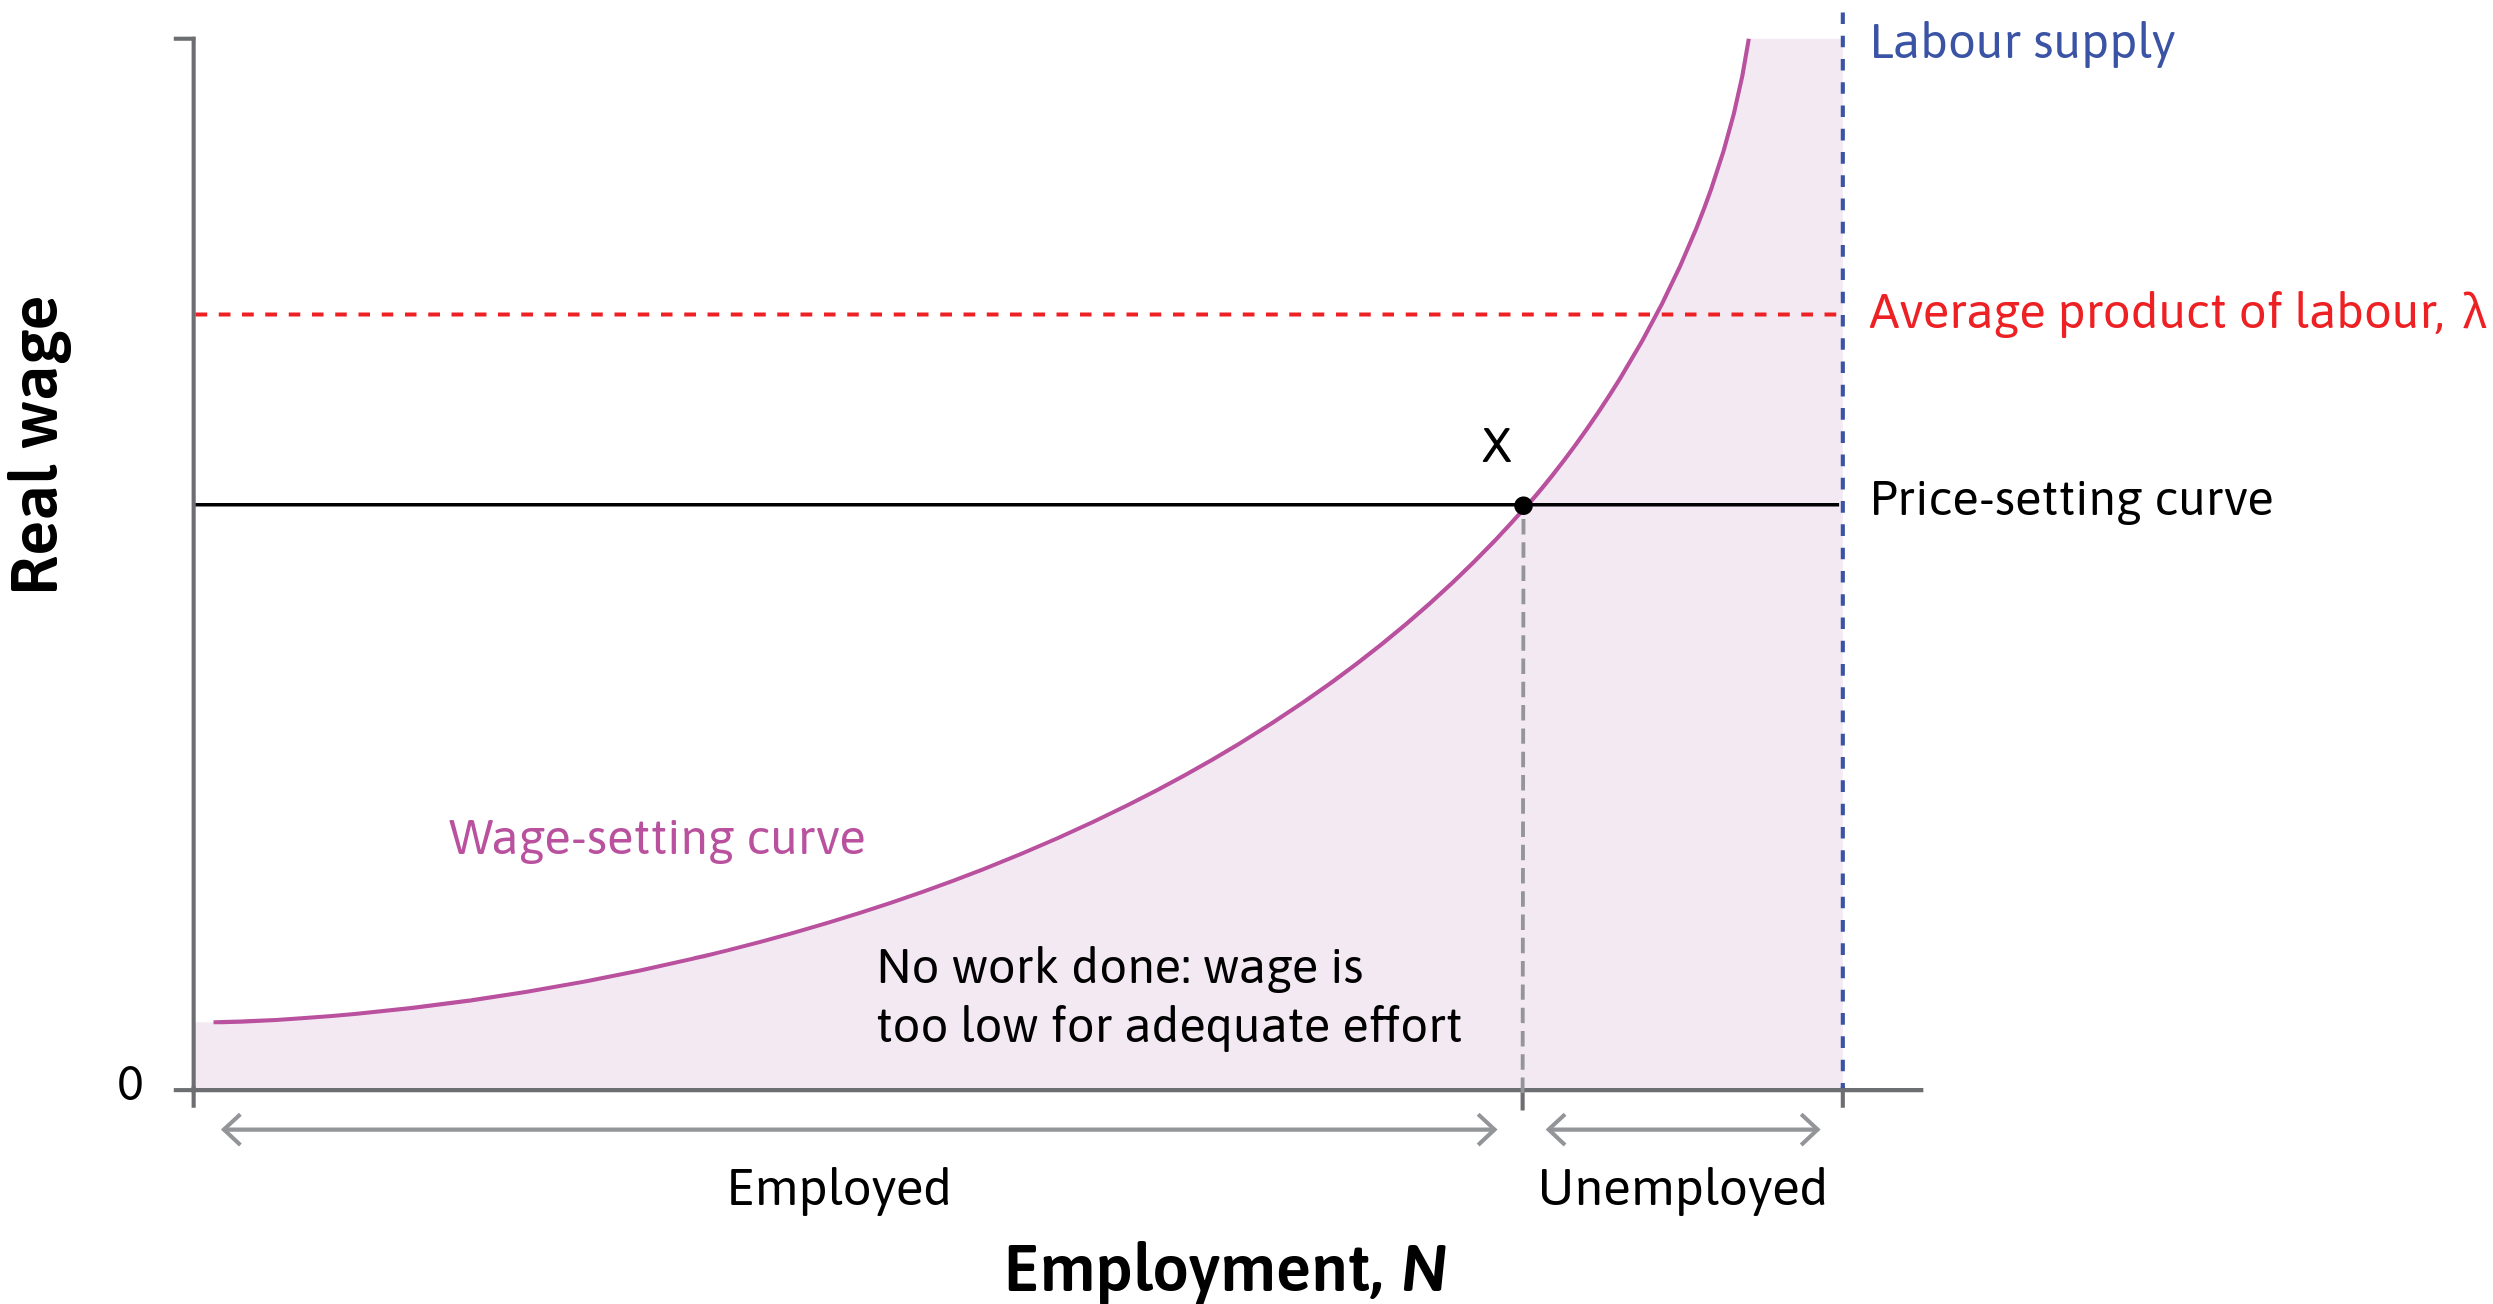
\includegraphics[width=\textwidth]{./figures/LaborMarketEq.png}
    \end{figure}
\end{frame}

\begin{frame}{Labor Market Equilibrium: Each Agent Explained}
\label{slide:Labor_Market_Equilibrium__Each_Agent_Explained}
    All parties are doing the best they can, given what everyone else is doing:
    \begin{itemize}
        \item The firms are offering the least wage to ensure workers’ effort
        \item Employment is the highest it can be, given the wage
        \item Those who have jobs cannot improve their situation by asking for higher pay or working less hard
        \item Those who do not have jobs would like to work, but cannot persuade firms to hire them by accepting lower wage (labour discipline concerns)
    \end{itemize}

\end{frame}

\begin{frame}{Involuntary unemployment}
\label{slide:Involuntary_unemployment}
    \begin{center}
        Unemployment = excess supply in the labour market
    \end{center}


There will always be unemployment in labour market equilibrium
\begin{itemize}
    \item No unemployment → zero cost of job loss → no effort
    \item Therefore some unemployment is necessary to motivate workers
    \item These are the involuntarily unemployed
\end{itemize}

\end{frame}

\section[Policy]{Policy Implications}
\label{sec:Policy_Implications}


\begin{frame}[allowframebreaks]{Demand-Deficient Unemployment: Model vs Real World}
\label{slide:Demand_Deficient_Unemployment__Model_v_s__Real_World}
    The increase in unemployment caused by the \alert{fall in aggregate demand} is called \textbf{demand-deficient unemployment}.

        \begin{figure}
            \centering
            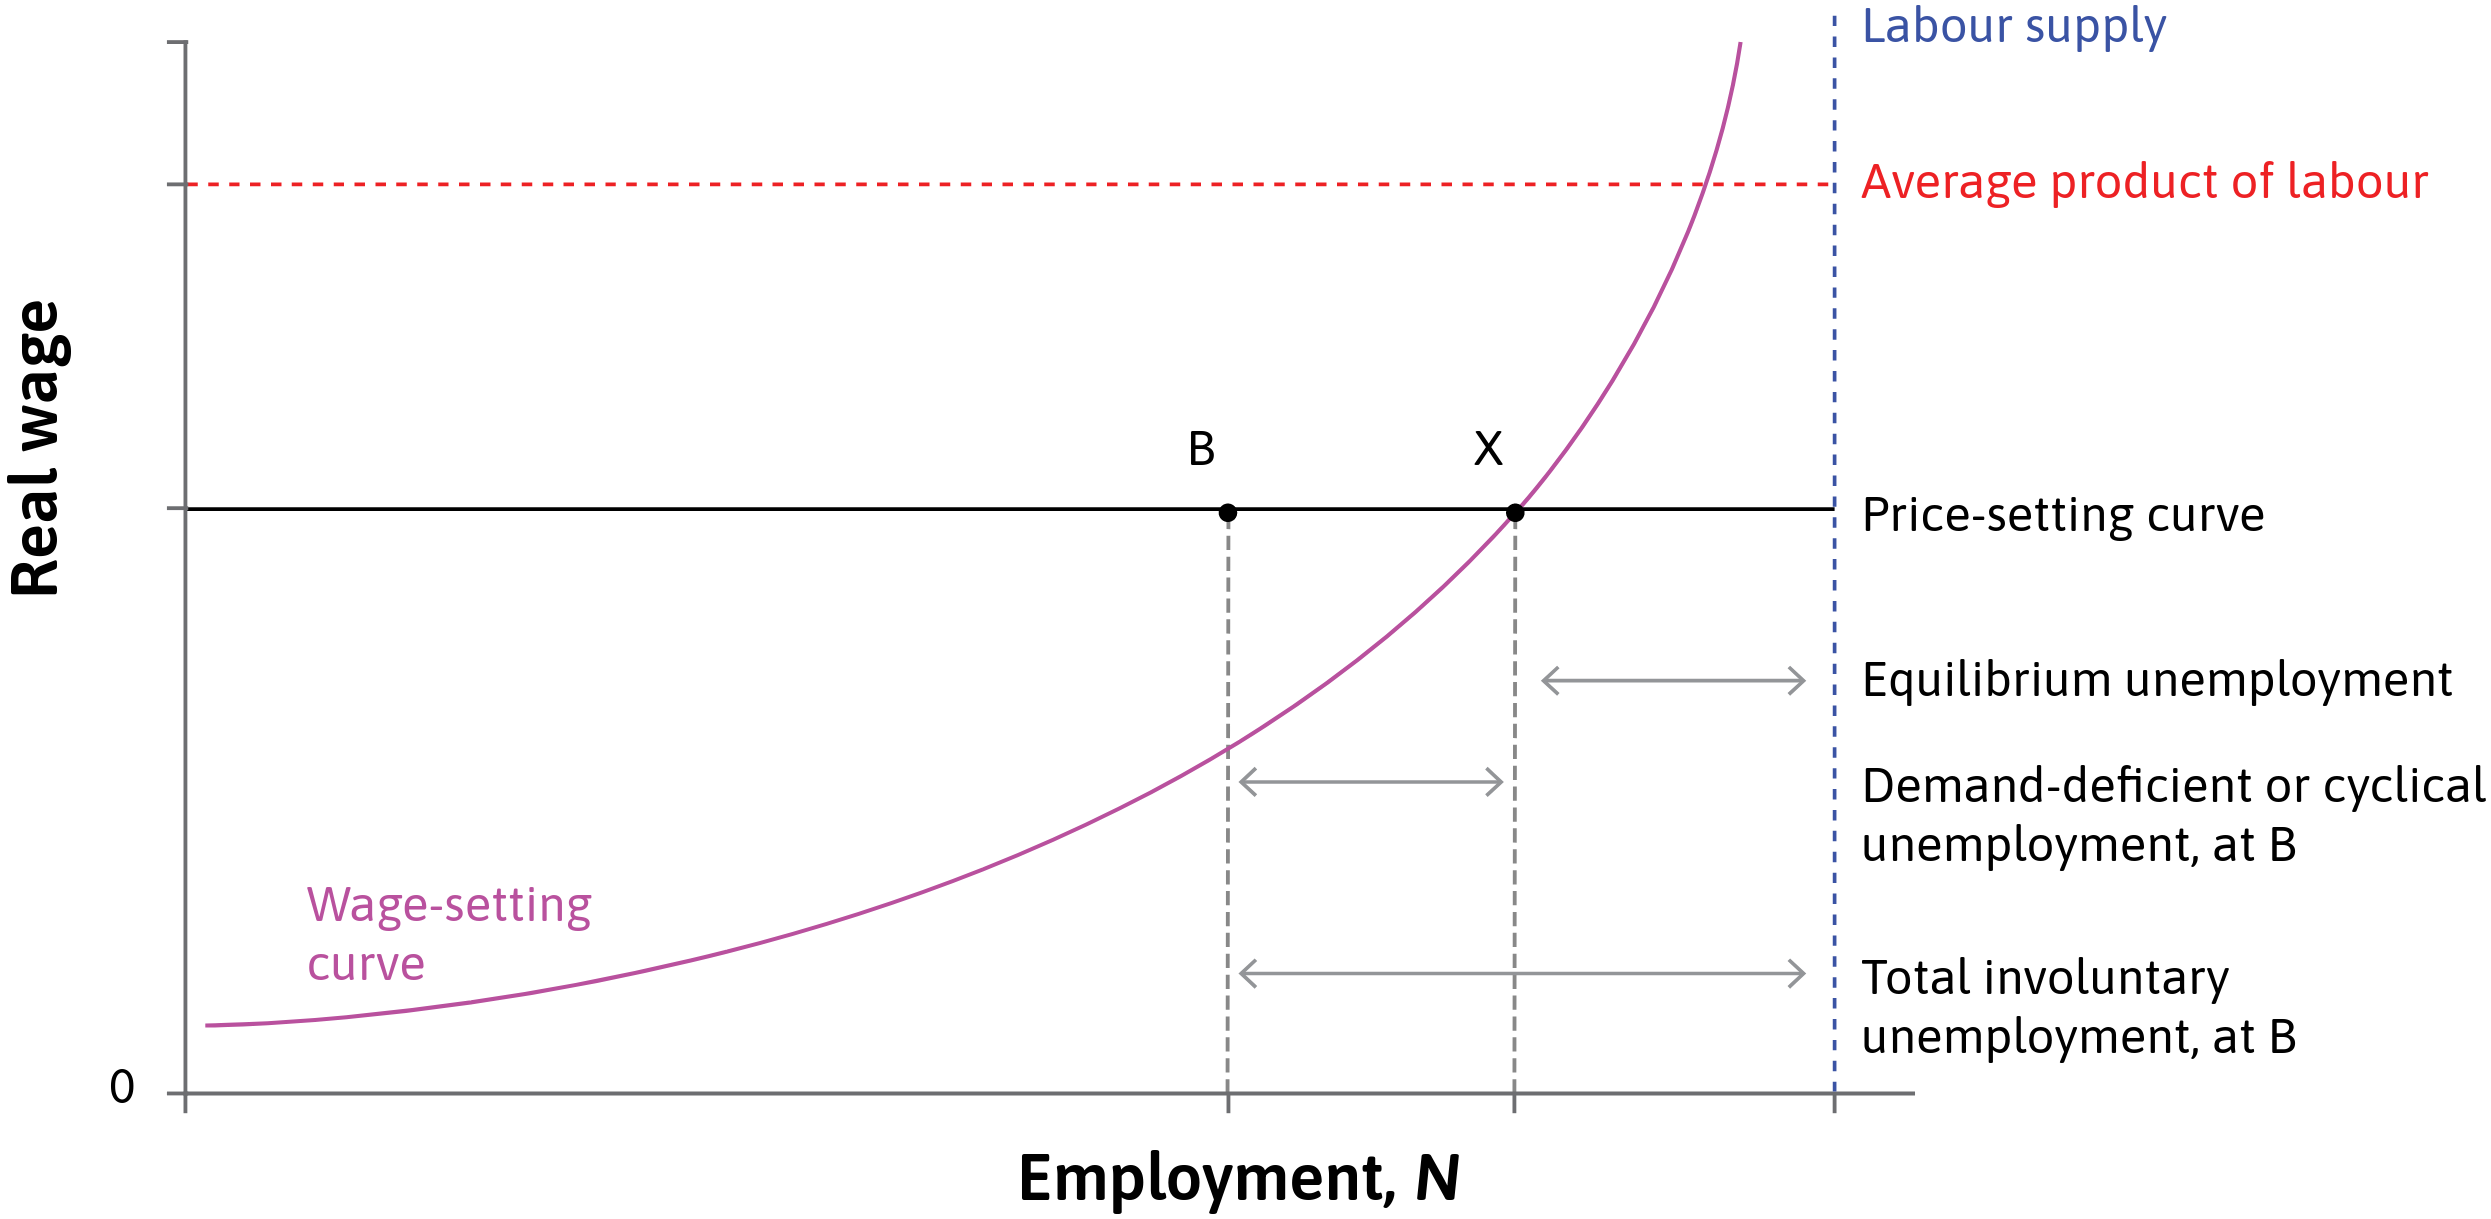
\includegraphics[width=\textwidth]{./figures/DemandDeficientUnemployment.png}
        \end{figure}

    \framebreak

    \begin{columns}
        \begin{column}{0.4\textwidth}
            \begin{itemize}
                \item What should firm react? (Remember we assume $ MC = AC $)
                \item If we are at point B, which means that \alert{prices is too high}
            \end{itemize}
        \end{column}
        \begin{column}{0.6\textwidth}
            \begin{figure}
                \centering
                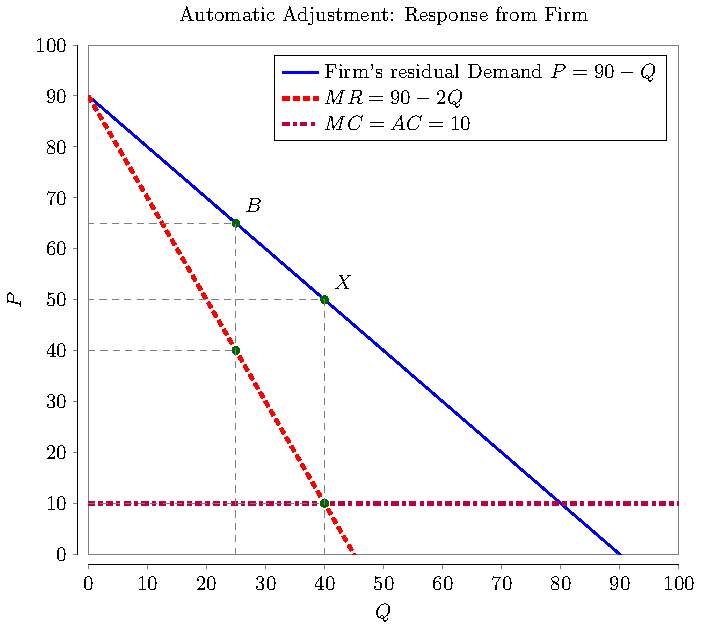
\includegraphics [width=\textwidth]{./figures/build/MRMC.pdf}
            \end{figure}
        \end{column}
    \end{columns}
    \framebreak
    \begin{itemize}
        \item Firms could lower wages without lowering workers’ effort
        \item Lower wages allow them to cut their prices
        \item Lower prices stimulate demand → output rises
        \item Firms hire more workers to produce more
        \item ... unemployment falls back to X
    \end{itemize}

    \framebreak

    Real economies do not function so smoothly:
    \begin{itemize}
        \item Workers resist cuts to their nominal wage (lower morale, strikes)
        \item Lower wages means people spend less → aggregate demand falls further
        \item Falling prices across the economy may lead consumers to postpone their purchases in hope to get even better bargain later
    \end{itemize}

\end{frame}

\begin{frame}{Government intervention}
\label{slide:Government_intervention}

            The government could increase its own spending (monetary \& fiscal policy) to expand aggregate demand.
             At B, firms would find it optimal to \textbf{produce more} (and hire more workers) instead of reducing wages.
            \begin{figure}
                \centering
                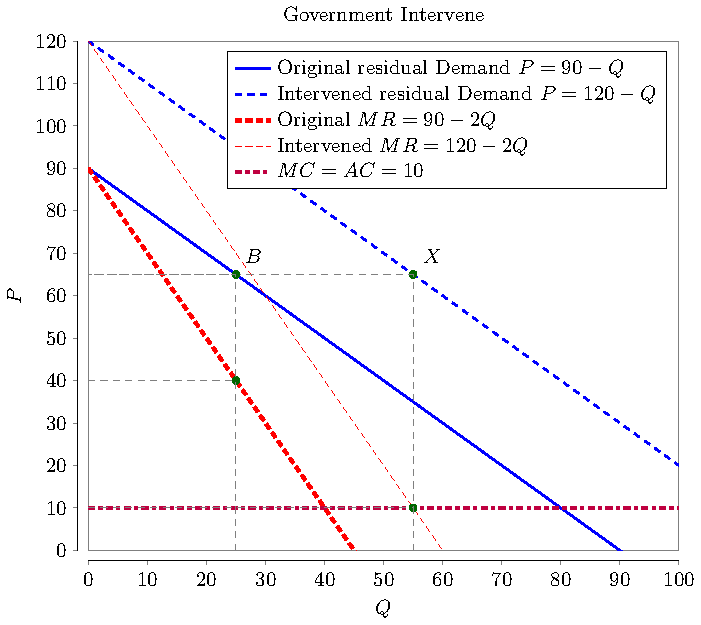
\includegraphics [width=0.6\textwidth]{./figures/build/GovIntervene.pdf}
            \end{figure}
\end{frame}

\begin{frame}{Immigration}
\label{slide:Immigration}
    Figures: \alert{\url{https://tinyurl.com/yr43j9v9}}
    \begin{figure}
        \centering
        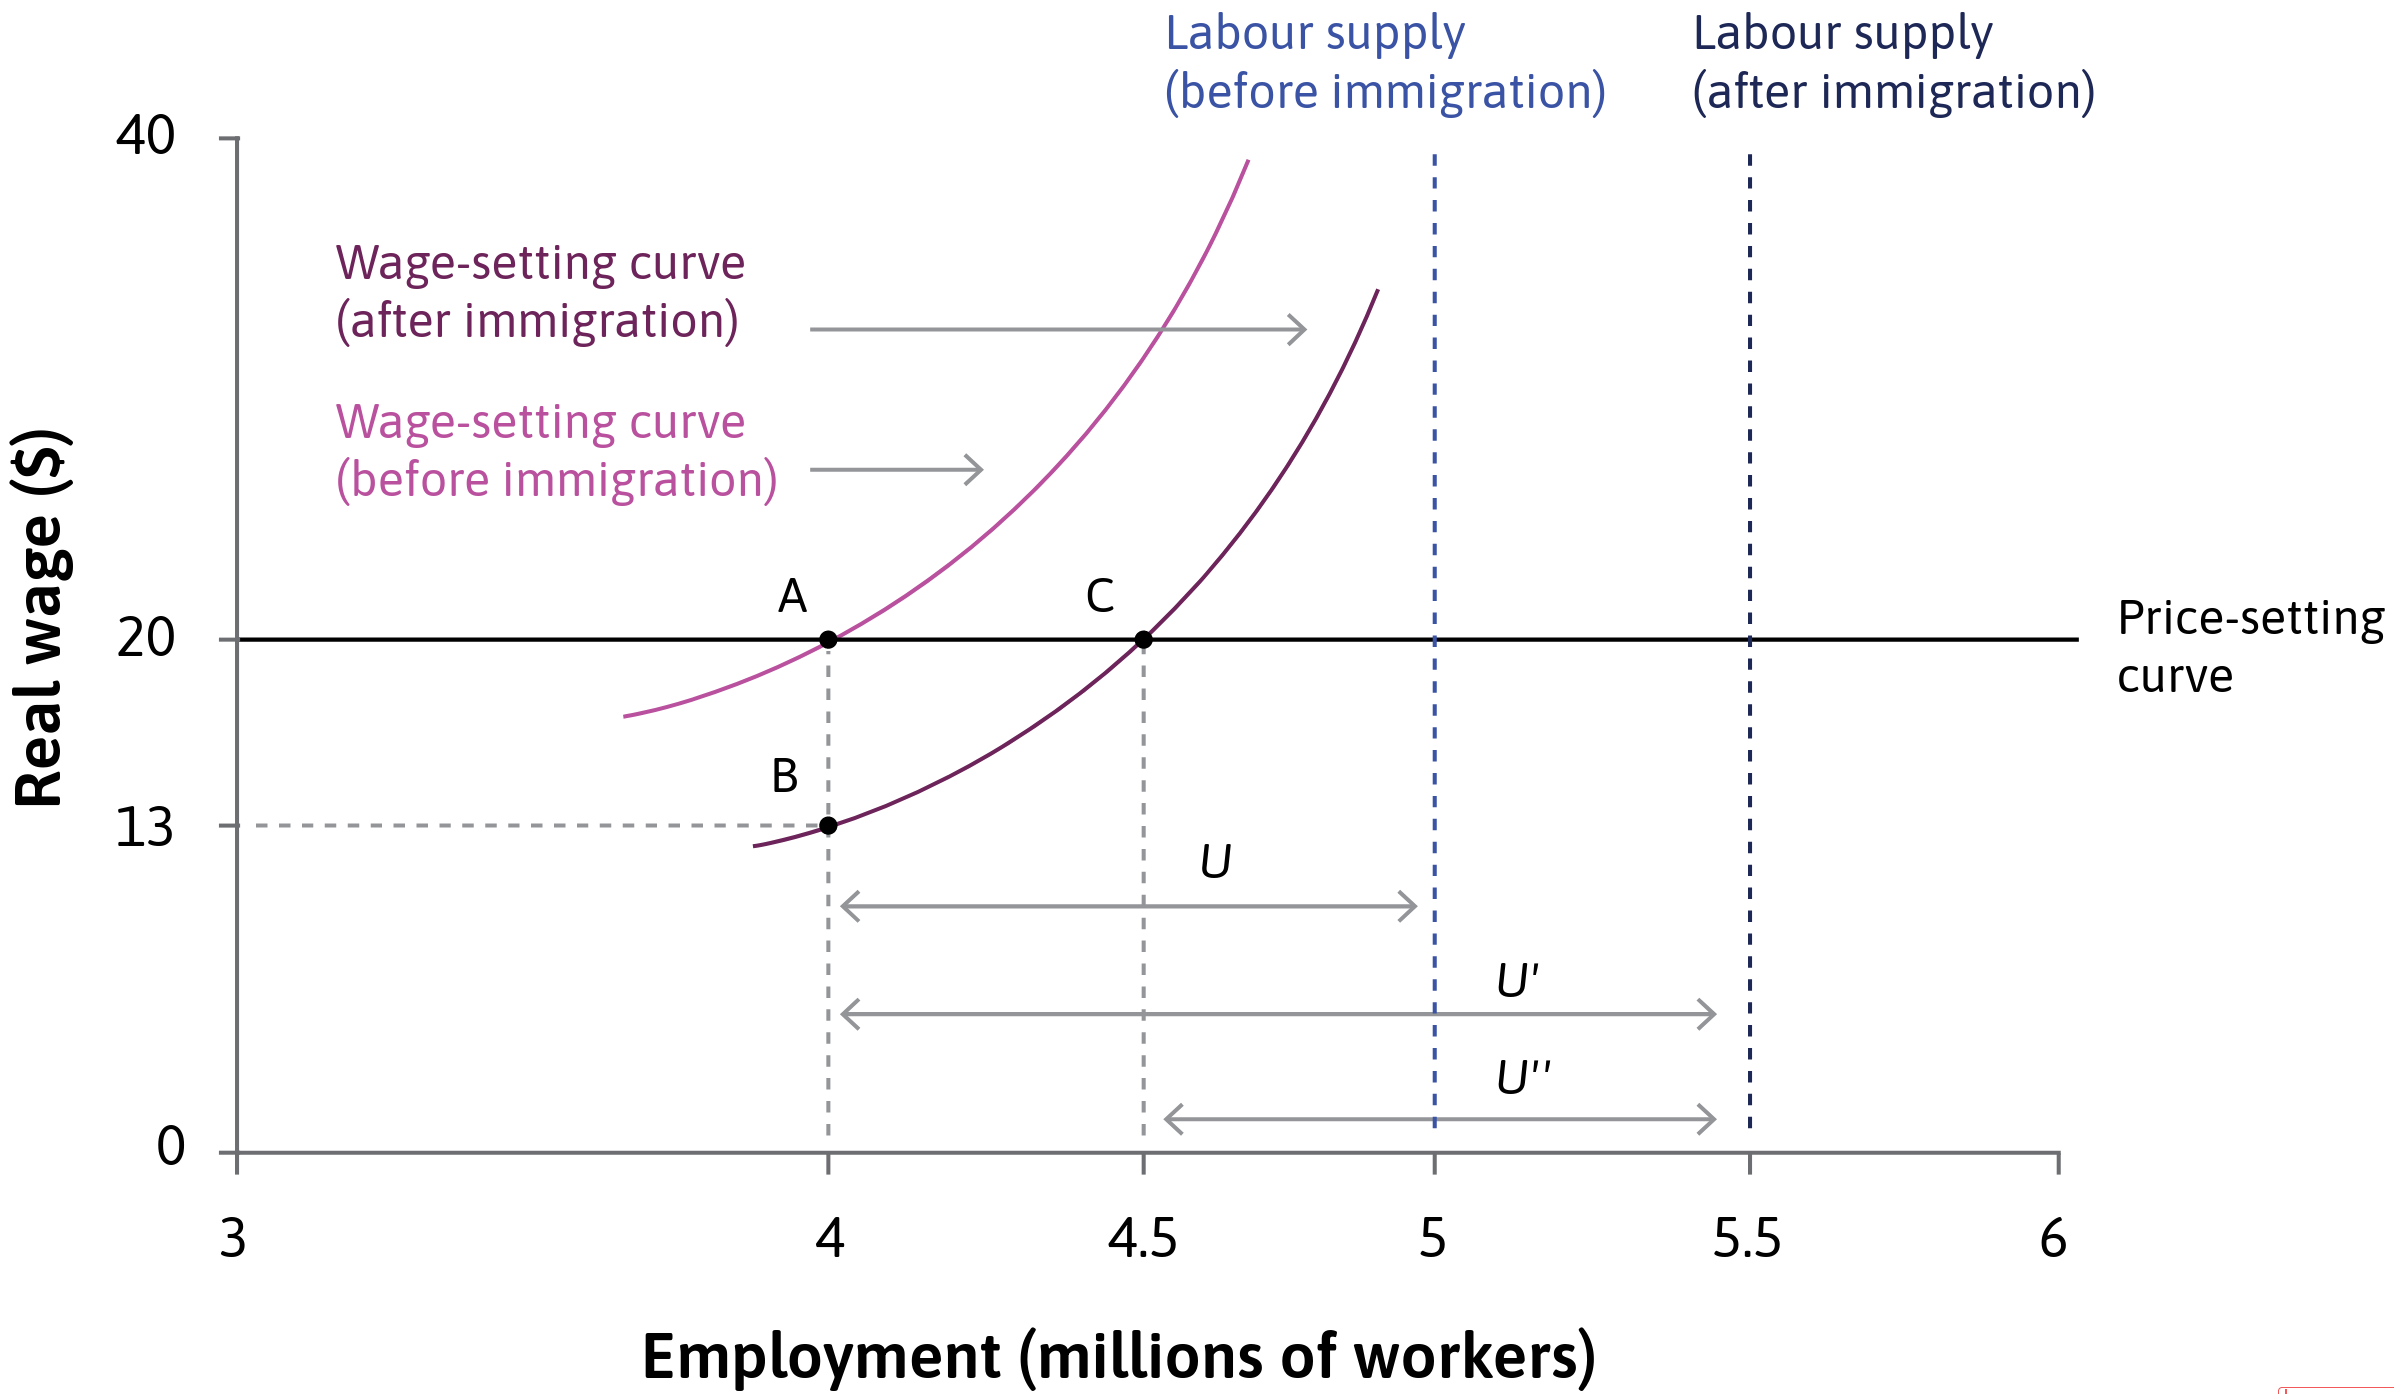
\includegraphics[width=\textwidth]{./figures/Immigration.png}
    \end{figure}

\end{frame}

\begin{frame}[allowframebreaks]{Labor Union: Model vs Real World}
\label{slide:Labor_Union}
    \begin{itemize}
        \item Labor union is an organization consisting predominantly of employees. Its main activities include the negotiation of rates of pay and conditions of employment for its members.
        \item Bargaining power of worker $ \uparrow  $ $ \Rightarrow  $ wage-setting curve shift \textbf{left} $ \Rightarrow  $ unemployment rate $ \uparrow  $
    \end{itemize}
    \begin{figure}
        \centering
        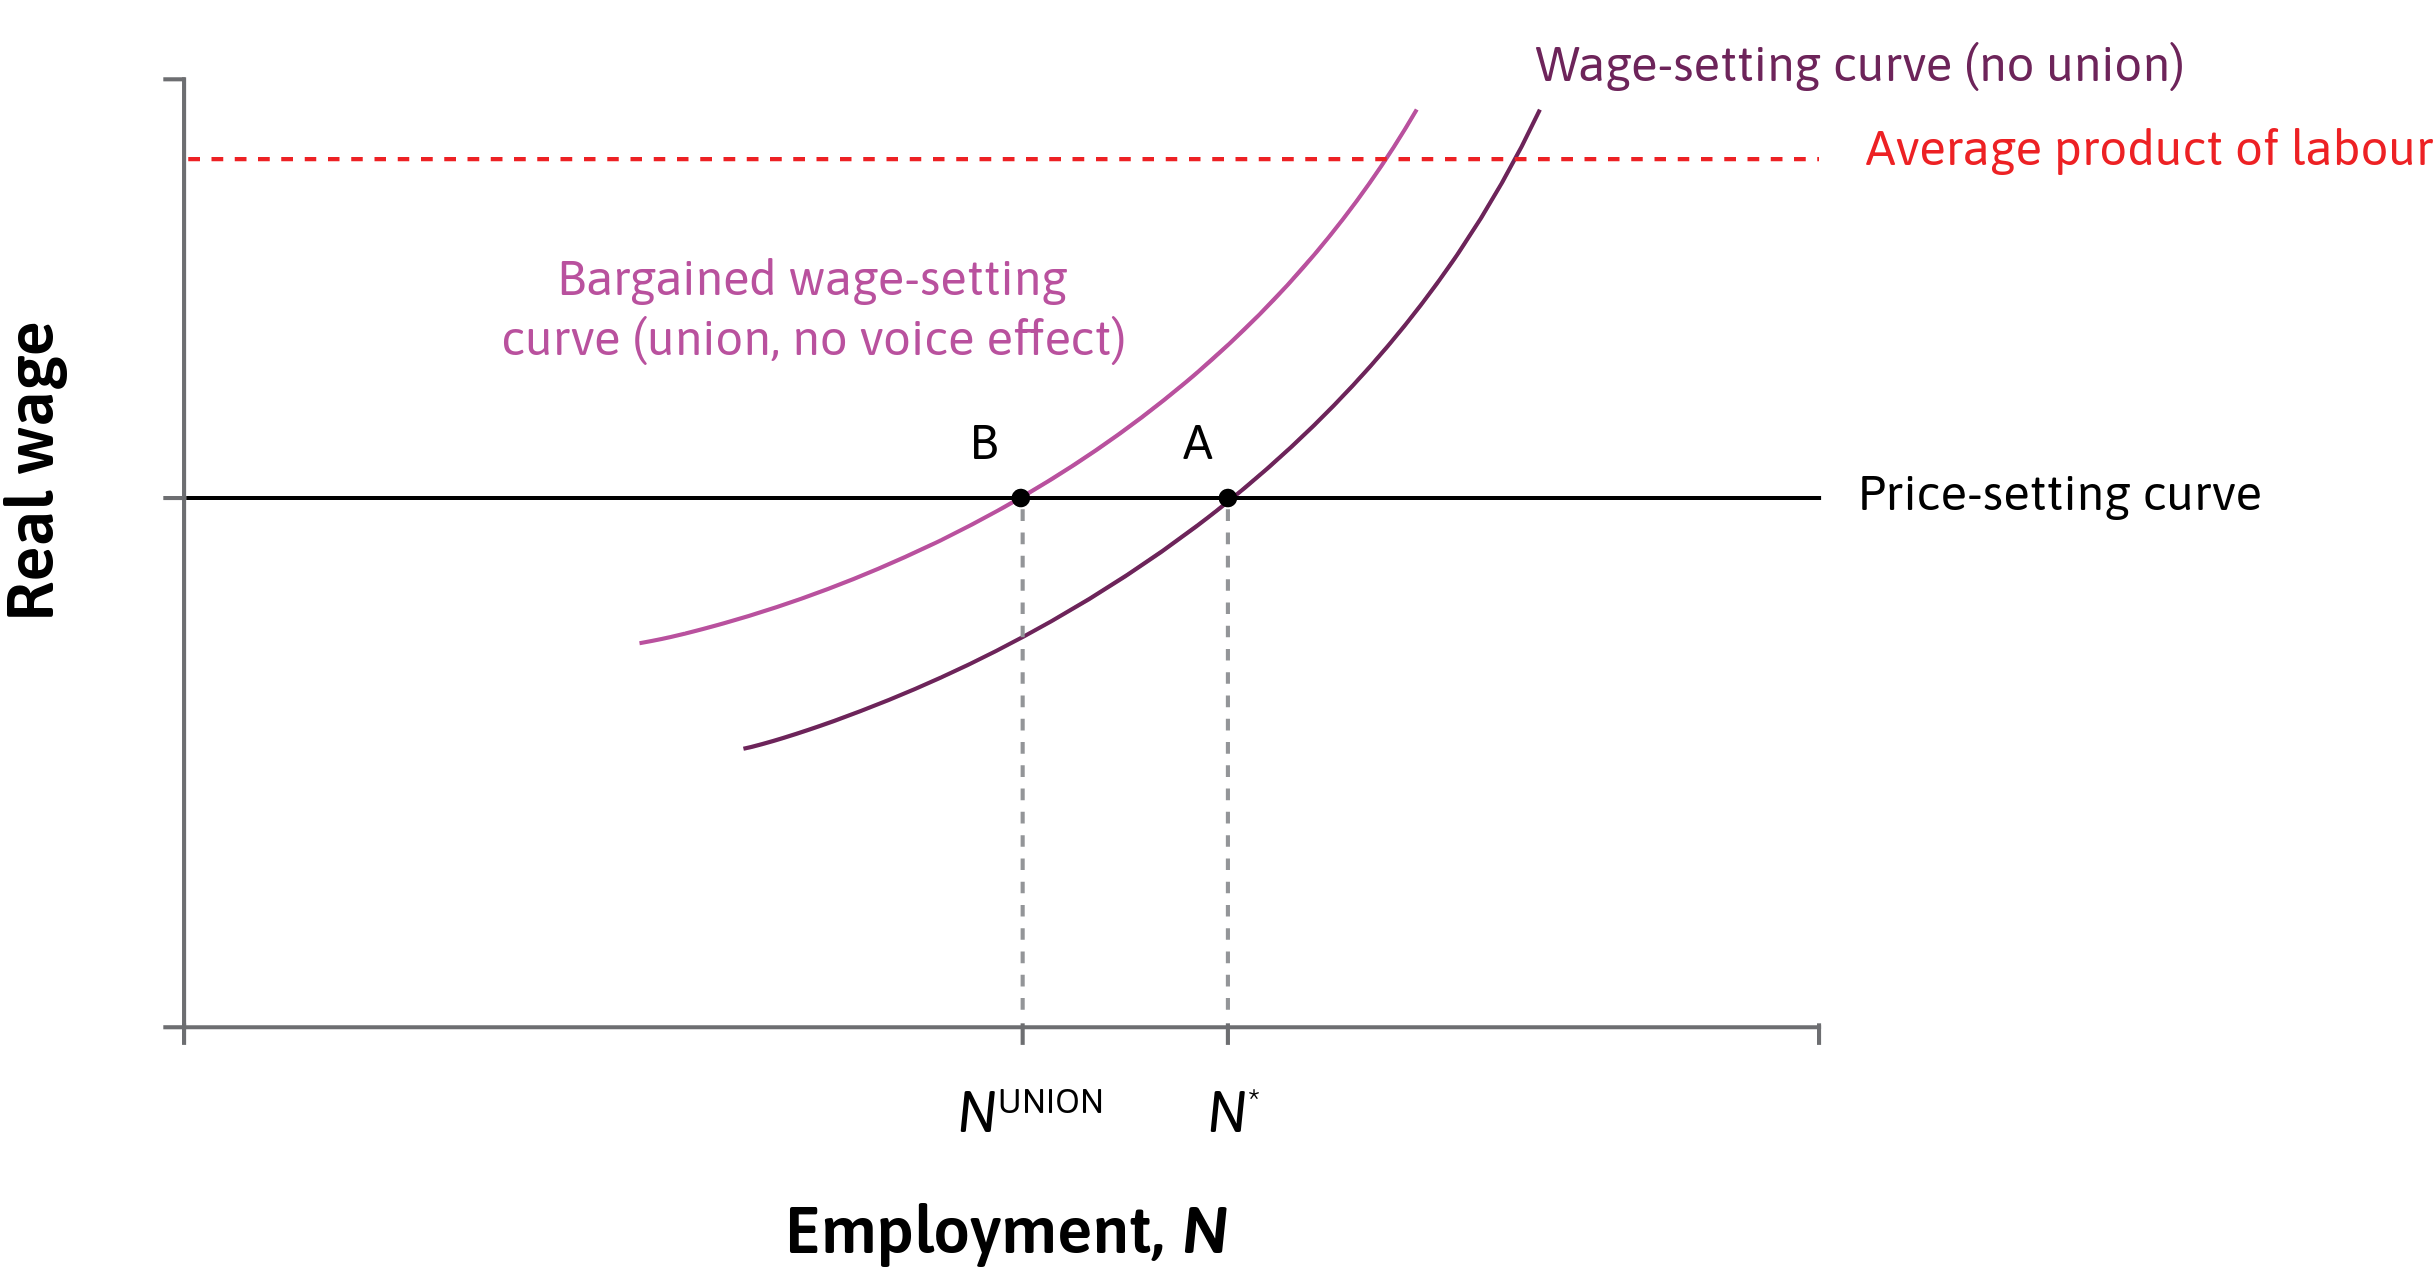
\includegraphics[width=0.6\textwidth]{./figures/LaborUnion_1.png}
    \end{figure}

    \framebreak

    \begin{itemize}
        \item But data says the opposite:
    \end{itemize}
    \begin{figure}
        \centering
        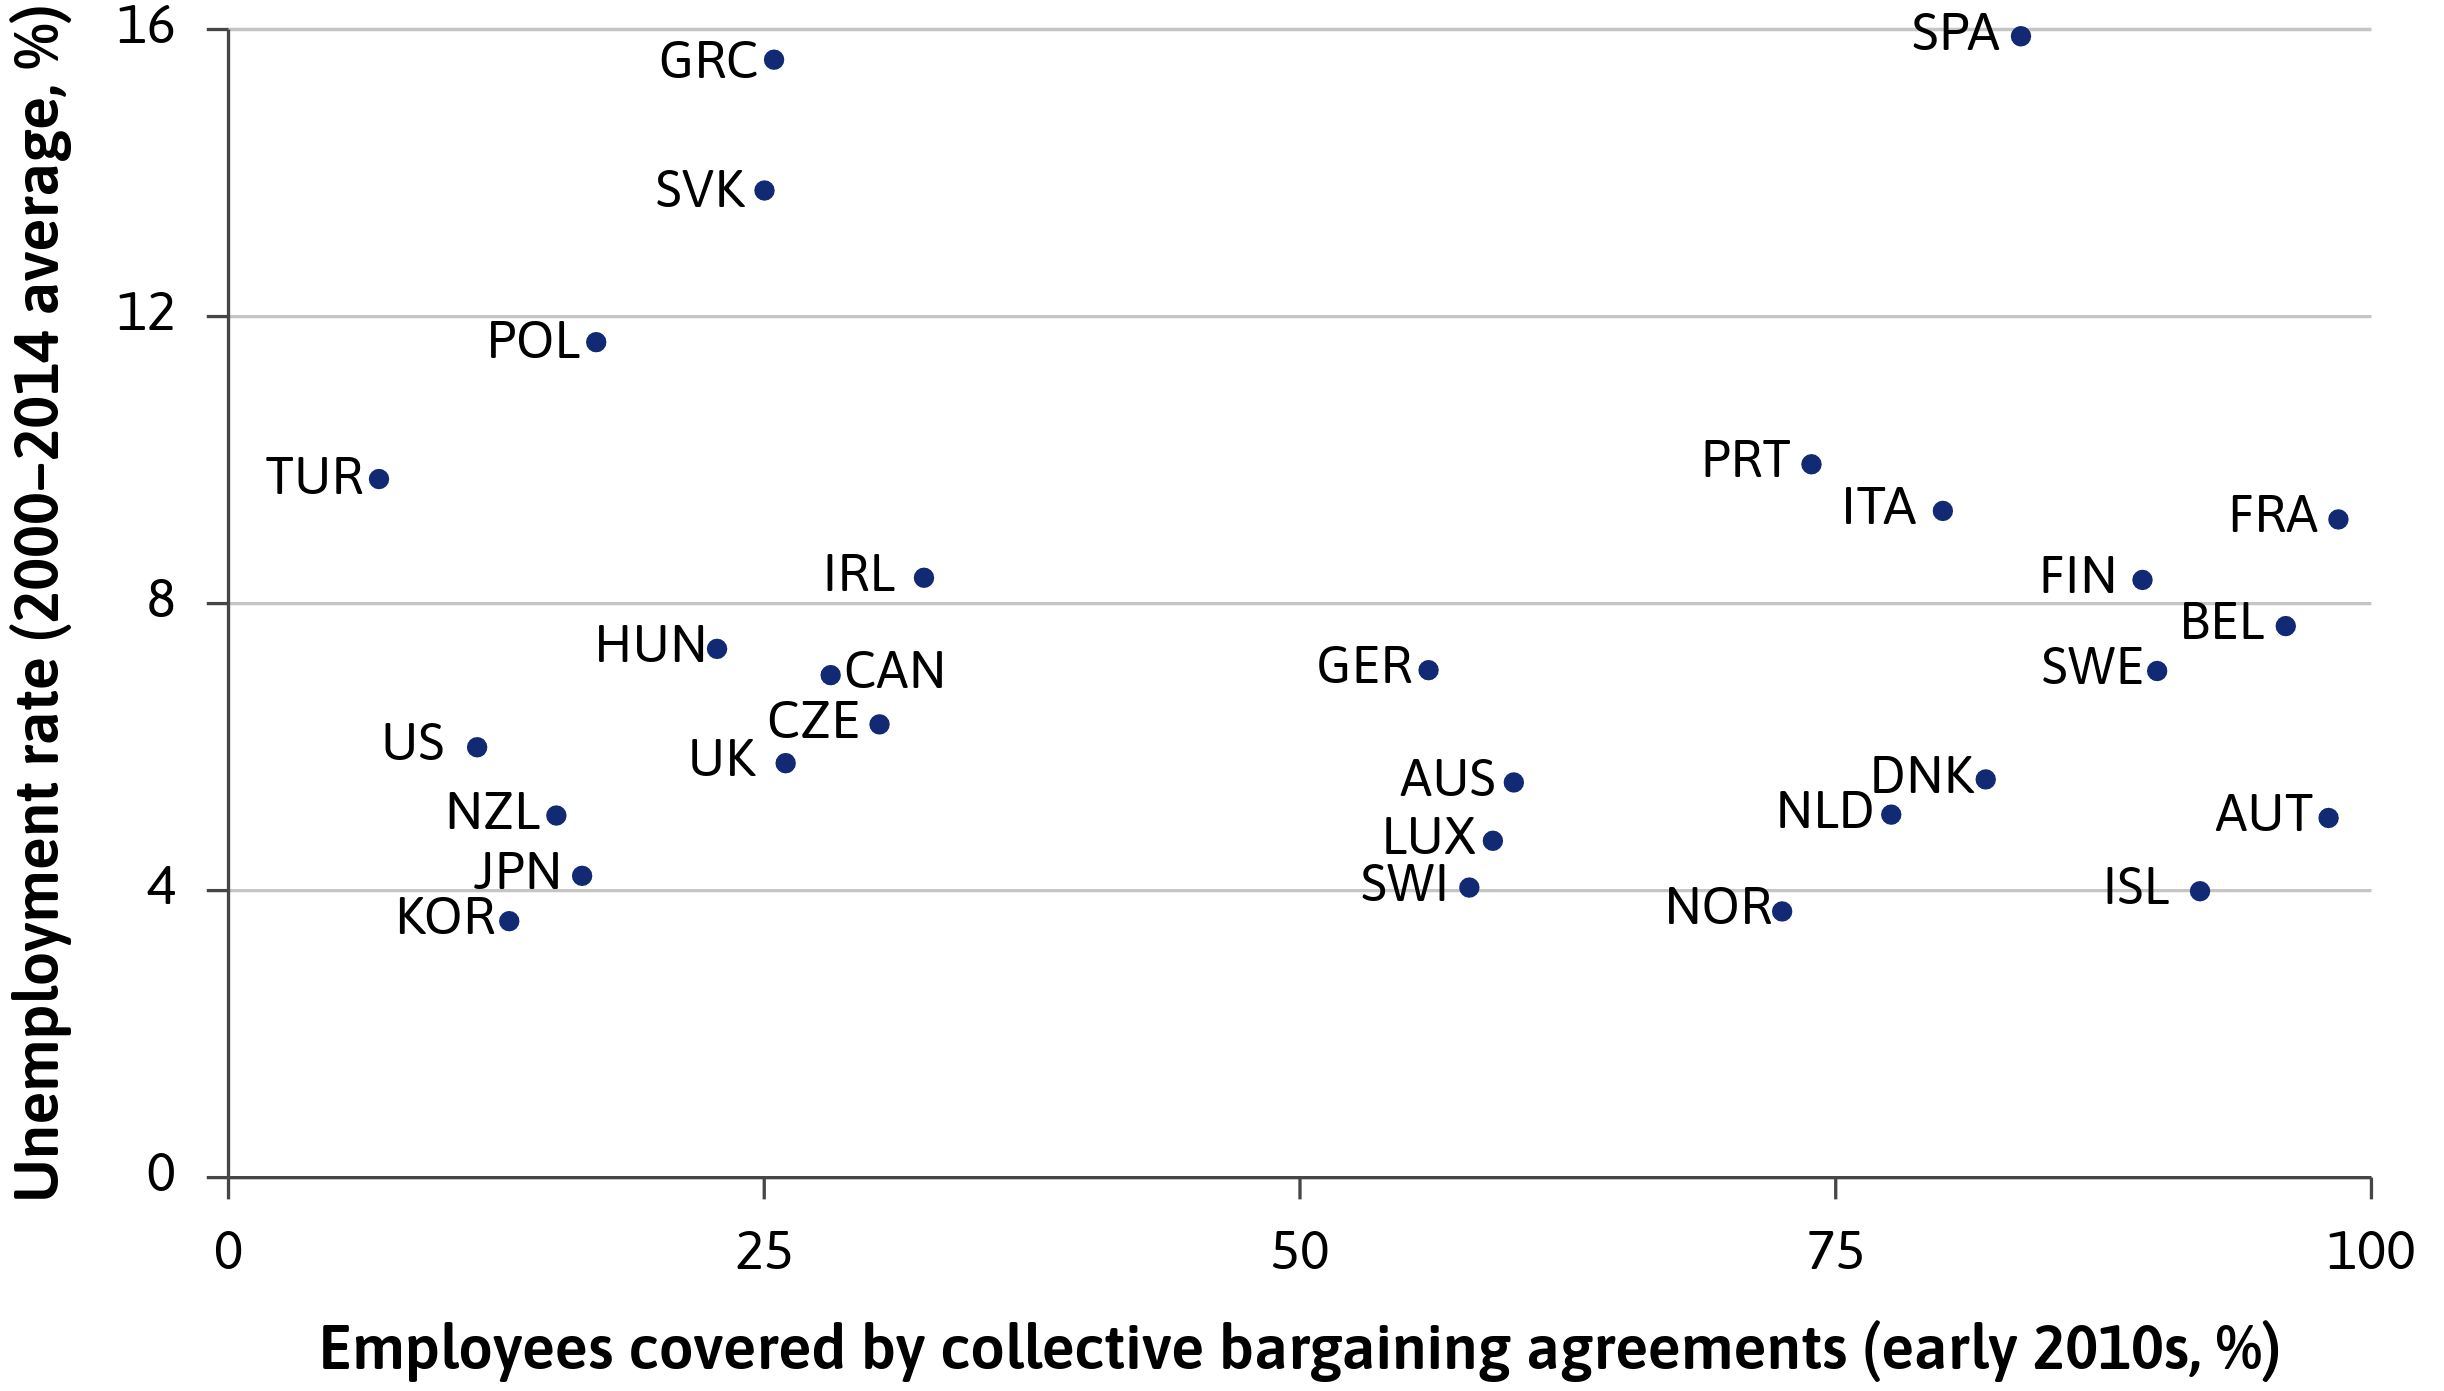
\includegraphics[width=0.8\textwidth]{./figures/LaborUnion_2.png}
    \end{figure}

    \framebreak

    Why? Textbook says the \alert{union voice effect}: Providing employees with a voice in how decisions are made may induce them to provide \alert{more effort for the same wage}.

    \begin{center}
        Really? 
\includegraphics[width=3em]{./figures/build/shrug.pdf}
    \end{center}


\end{frame}

\begin{frame}{Summary for Policies}
\label{slide:Summary_for_Policies}
    \begin{itemize}
        \item Shifts in the price-setting curve:
        \begin{enumerate}
            \item Education \& training: labour productivity ↑
            \item Wage subsidy: Production costs and prices ↓
        \end{enumerate}
        \item Shifts in the wage-setting curve:
        \begin{enumerate}
            \item Lower unemployment benefit: reservation wage ↓
        \end{enumerate}
        \item Shifts in labour supply curve:
        \begin{enumerate}
            \item immigration policies: labour supply ↑
            \item childcare provision: female labour participation ↑
        \end{enumerate}
    \end{itemize}
\end{frame}




\section{Appendix}
\label{sec:Appendix}

\appendix
% -------------------------------------------
\setbeamertemplate{headline}
{
\setbeamercolor{section in head/foot}{fg=black, bg=white}
\vskip1em \tiny \insertsectionnavigationhorizontal{1\paperwidth}{\hspace{0.50\paperwidth}}{}
}
%------------------------------------------
% \begin{frame}\frametitle{}
% \begin{columns}
% \label{Appendix}
% \column{1\linewidth}
% \centering
% {\Large \alert{Appendix}}
% \end{columns}
% \end{frame}
%------------------------------------------
\begin{frame}{What functional form of cost function allow $ MC = AC $?}
\label{slide:What_functional_form_of_cost_function_allow___MC___AC___}

\jump{slide:Derivation_of_Price_setting_curve}{Back}

The general form of cost function is $ C(Q) = a Q^{b} + c $, so to make $ MC(Q) = AC(Q) $, we need
%
\begin{align*}
    MC(Q)
        & = AC(Q)
    \\
    \frac{\partial C(Q)}{\partial Q}
        & = \frac{C(Q)}{Q}
    \\
    a b Q^{b-1}
        & = a Q^{b-1} + \frac{c}{Q}
\end{align*}
%
So the easiest way to force $ MC = AC $ is unsurprisingly, $ b = 1 $ and $c = 0 $, i.e., a flat line.

    \begin{center}
        
\includegraphics[width=3em]{./figures/build/shrug.pdf}
    \end{center}
\end{frame}


\end{document}
